\documentclass[10pt,a4paper]{article}
\usepackage[utf8]{inputenc}
\usepackage[T1]{fontenc}
\usepackage{helvet}
\renewcommand{\familydefault}{\sfdefault}
\usepackage[margin=0.7in,top=0.8in,bottom=0.8in]{geometry}
\usepackage{amsmath,amssymb}
\usepackage{graphicx}
\usepackage[table,xcdraw]{xcolor}
\usepackage{booktabs}
\usepackage{tabularx}
\usepackage{array}
\usepackage{enumitem}
\usepackage{titlesec}
\usepackage{fancyhdr}
\usepackage{lastpage}
\usepackage{tcolorbox}
\tcbuselibrary{skins,breakable}
\usepackage{tikz}
\usetikzlibrary{positioning,calc,shapes.geometric,decorations.pathmorphing,backgrounds,patterns}
\usepackage{fontawesome5}
\usepackage{hyperref}

% Define color palette (both camelCase and UPPERCASE for titlesec compatibility)
\definecolor{NavyPrimary}{HTML}{0F172A}
\definecolor{NAVYPRIMARY}{HTML}{0F172A}
\definecolor{TealSecondary}{HTML}{0284C7}
\definecolor{TEALSECONDARY}{HTML}{0284C7}
\definecolor{SlateDark}{HTML}{334155}
\definecolor{SLATEDARK}{HTML}{334155}
\definecolor{LightBg}{HTML}{F8FAFC}
\definecolor{LIGHTBG}{HTML}{F8FAFC}
\definecolor{BorderGrey}{HTML}{E2E8F0}
\definecolor{AmberAccent}{HTML}{D97706}
\definecolor{GreenPass}{HTML}{16A34A}
\definecolor{RedRisk}{HTML}{DC2626}

% Hyperref setup
\hypersetup{
    colorlinks=true,
    linkcolor=TealSecondary,
    urlcolor=TealSecondary,
    citecolor=TealSecondary
}

% Page style setup
\pagestyle{fancy}
\fancyhf{}
\rhead{\footnotesize \textcolor{SlateDark}{\textbf{BAA-DARPA-I2O-2026-09} \ \textbar\ \ Technical \& Cost Proposal}}
\lhead{\footnotesize \textcolor{SlateDark}{\textbf{UNCLASSIFIED // FOR OFFICIAL USE ONLY}}}
\lfoot{\footnotesize \textcolor{SlateDark}{Apex Defense Systems, Inc. --- Project HYPERION}}
\rfoot{\footnotesize \textcolor{SlateDark}{Page \thepage\ of \pageref{LastPage}}}
\renewcommand{\headrulewidth}{0.4pt}
\renewcommand{\footrulewidth}{0.4pt}

% Section formatting
\titleformat{\section}
  {\color{NavyPrimary}\large\bfseries}
  {\thesection.}{0.5em}{\MakeUppercase}
  [\color{TealSecondary}\titlerule]

\titleformat{\subsection}
  {\color{TealSecondary}\normalsize\bfseries}
  {\thesubsection}{0.5em}{}

\titleformat{\subsubsection}
  {\color{NavyPrimary}\small\bfseries}
  {\thesubsubsection}{0.5em}{}

\titlespacing*{\section}{0pt}{9pt}{3pt}
\titlespacing*{\subsection}{0pt}{7pt}{2pt}
\titlespacing*{\subsubsection}{0pt}{5pt}{2pt}

% Tcolorbox custom styles
\tcbset{
  proposalbox/.style={
    enhanced,
    colback=LightBg,
    colframe=NavyPrimary,
    arc=3pt,
    boxrule=0.8pt,
    fonttitle=\bfseries\color{white},
    coltitle=white,
    colbacktitle=NavyPrimary,
    top=5pt,bottom=5pt,left=8pt,right=8pt
  },
  cardbox/.style={
    enhanced,
    colback=white,
    colframe=BorderGrey,
    arc=2pt,
    boxrule=0.6pt,
    top=5pt,bottom=5pt,left=7pt,right=7pt
  },
  metricbox/.style={
    enhanced,
    colback=LightBg,
    colframe=TealSecondary,
    arc=2pt,
    boxrule=0.8pt,
    top=4pt,bottom=4pt,left=4pt,right=4pt,
    halign=center
  }
}

\begin{document}

% ---------------------------------------------------------
% COVER HEADER BLOCK
% ---------------------------------------------------------
\begin{tcolorbox}[proposalbox, title={\Large\faShield* \ \ DARPA TECHNICAL \& COST PROPOSAL}]
\vspace{1pt}
{\Large\bfseries\color{NavyPrimary} PROJECT HYPERION: Zero-Trust Adaptive Mesh Neural Routing for Contested Electromagnetic Environments}

\vspace{4pt}
\hrule height 0.5pt color BorderGrey
\vspace{4pt}

\small
\begin{tabularx}{\linewidth}{@{}l X l X@{}}
\textbf{BAA Number:} & BAA-DARPA-I2O-2026-09 & \textbf{Submitting Org:} & Apex Defense Systems, Inc. \\
\textbf{Technical Topic:} & Resilient Tactical Comms & \textbf{Team Partners:} & Vertex Labs, Meridian Micro \\
\textbf{Principal Investigator:} & Dr. Marcus Vance & \textbf{Period of Perf.:} & 24 Months (Base + Option) \\
\textbf{PI Contact Email:} & m.vance@apexdef.com & \textbf{Total Proposed Cost:} & \$3,845,200 (CPFF Contract) \\
\end{tabularx}
\end{tcolorbox}

\vspace{4pt}

% Quick Metrics Bar
\noindent
\begin{minipage}[t]{0.235\linewidth}
  \begin{tcolorbox}[metricbox]
    {\scriptsize\bfseries\color{SlateDark} TOTAL BUDGET}\\[2pt]
    {\large\bfseries\color{NavyPrimary} \$3,845,200}
  \end{tcolorbox}
\end{minipage}%
\hfill
\begin{minipage}[t]{0.235\linewidth}
  \begin{tcolorbox}[metricbox]
    {\scriptsize\bfseries\color{SlateDark} PERFORMANCE PERIOD}\\[2pt]
    {\large\bfseries\color{TealSecondary} 24 Months}
  \end{tcolorbox}
\end{minipage}%
\hfill
\begin{minipage}[t]{0.235\linewidth}
  \begin{tcolorbox}[metricbox]
    {\scriptsize\bfseries\color{SlateDark} TARGET MATURITY}\\[2pt]
    {\large\bfseries\color{NavyPrimary} TRL 3 $\rightarrow$ TRL 6}
  \end{tcolorbox}
\end{minipage}%
\hfill
\begin{minipage}[t]{0.235\linewidth}
  \begin{tcolorbox}[metricbox]
    {\scriptsize\bfseries\color{SlateDark} SECURITY CLEARANCE}\\[2pt]
    {\large\bfseries\color{AmberAccent} TOP SECRET / SCI}
  \end{tcolorbox}
\end{minipage}

\vspace{6pt}

% ---------------------------------------------------------
% SECTION 1: EXECUTIVE SUMMARY
% ---------------------------------------------------------
\section{Executive Summary \& Proposal Overview}

Modern tactical operations encounter unprecedented electromagnetic spectrum (EMS) warfare, characterized by high-powered directional jamming, cognitive RF spoofing, and instantaneous node compromise. Legacy military ad-hoc networks (MANETs) rely on centralized route discovery and predictable frequency hopping schedules, leaving tactical units vulnerable to total communication blackouts within seconds of adversarial engagement.

\textbf{Project HYPERION} directly addresses this critical vulnerability by introducing a decentralized, zero-trust neuromorphic routing architecture. Designed for deployment at the tactical edge, HYPERION leverages embedded low-power tensor processing units (TPUs) to dynamically synthesize interference-free communication channels in real time without relying on GPS, fixed infrastructure, or centralized command nodes.

\vspace{4pt}

\noindent
\begin{minipage}[t]{0.485\linewidth}
  \begin{tcolorbox}[cardbox]
    \textbf{\color{NavyPrimary}\faMicrochip \ \ Key Innovation 1: Edge Neural Spectrum Synthesis}
    \vspace{2pt}
    \begin{itemize}[leftmargin=11pt,label=\tiny$\blacksquare$,itemsep=1pt]
      \item Real-time RF spectrum sensing via deep reinforcement learning running at sub-50$\mu$s inference latency.
      \item Predicts adversarial jamming sweeps prior to channel degradation, initiating preemptive waveform synthesis.
      \item Zero dependency on satellite timing references or pre-shared hopping tables.
    \end{itemize}
  \end{tcolorbox}
\end{minipage}%
\hfill
\begin{minipage}[t]{0.485\linewidth}
  \begin{tcolorbox}[cardbox]
    \textbf{\color{NavyPrimary}\faLock \ \ Key Innovation 2: Cryptographic Zero-Trust Mesh}
    \vspace{2pt}
    \begin{itemize}[leftmargin=11pt,label=\tiny$\blacksquare$,itemsep=1pt]
      \item Micro-second zero-knowledge proof (ZKP) identity verification for every transmitted data packet.
      \item Instantaneous detection and isolation of compromised or spoofed friendly nodes within 1.2 milliseconds.
      \item Quantum-resistant lattice cryptography optimized for SWaP-constrained field radios.
    \end{itemize}
  \end{tcolorbox}
\end{minipage}

\vspace{4pt}

\subsection{Statement of Work \& High-Level Objectives}
Apex Defense Systems, in partnership with Vertex Research Laboratories and Meridian Microelectronics, proposes a 24-month effort structured in two distinct phases:
\begin{enumerate}[label=\textbf{Objective \arabic*:},leftmargin=65pt,itemsep=1pt]
  \item \textbf{Phase I (Base -- 12 Months):} Formulate and validate the HYPERION Neuromorphic Algorithm Suite, construct a high-fidelity Hardware-in-the-Loop (HITL) RF simulation rig, and demonstrate TRL 4 capability across a 20-node simulated mesh under heavy adversarial jamming.
  \item \textbf{Phase II (Option -- 12 Months):} Fabricate custom software-defined radio (SDR) mezzanine cards with Meridian TPU accelerators, integrate onto tactical unmanned aerial vehicles (UAVs) and ground units, and execute a live-fire field test achieving TRL 6 validation.
\end{enumerate}

\newpage

% ---------------------------------------------------------
% SECTION 2: TECHNICAL APPROACH & SYSTEM ARCHITECTURE
% ---------------------------------------------------------
\section{Technical Approach \& System Architecture}

\subsection{Operational Paradigm \& System Topology}
The HYPERION system architecture operates across three synchronized layers: the Physical RF Sensing Layer, the Neuromorphic Waveform Synthesis Layer, and the Zero-Trust Routing Fabric. Figure 1 illustrates the functional interaction between contested tactical nodes, edge TPU processing, and anti-jamming packet synthesis.

\vspace{3pt}

% TikZ System Architecture Diagram
\begin{center}
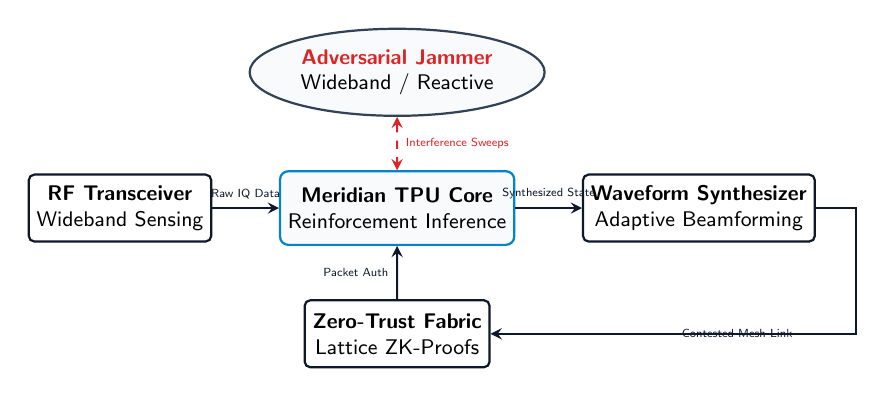
\begin{tikzpicture}[scale=0.85, transform shape,
  box/.style={rectangle, draw=NavyPrimary, fill=white, thick, minimum width=2.7cm, minimum height=1.0cm, align=center, rounded corners=2pt, font=\sffamily\small},
  tpu/.style={rectangle, draw=TealSecondary, fill=LightBg, thick, minimum width=3.0cm, minimum height=1.1cm, align=center, rounded corners=3pt, font=\sffamily\small},
  cloud/.style={ellipse, draw=SlateDark, fill=LightBg, thick, minimum width=2.4cm, minimum height=0.9cm, align=center, font=\sffamily\small},
  arrow/.style={->, >=stealth, thick, color=NavyPrimary},
  warnarrow/.style={<->, >=stealth, thick, color=RedRisk, dashed}
]

  % Nodes
  \node[box] (sensor) {\textbf{RF Transceiver}\\Wideband Sensing};
  \node[tpu, right=1.0cm of sensor] (tpu) {\textbf{Meridian TPU Core}\\Reinforcement Inference};
  \node[box, right=1.0cm of tpu] (synth) {\textbf{Waveform Synthesizer}\\Adaptive Beamforming};
  \node[cloud, above=0.8cm of tpu] (jam) {\color{RedRisk}\textbf{Adversarial Jammer}\\Wideband / Reactive};
  \node[box, below=0.8cm of tpu] (zkp) {\textbf{Zero-Trust Fabric}\\Lattice ZK-Proofs};

  % Connections
  \draw[arrow] (sensor) -- node[above, font=\tiny] {Raw IQ Data} (tpu);
  \draw[arrow] (tpu) -- node[above, font=\tiny] {Synthesized State} (synth);
  \draw[arrow] (zkp) -- node[left, font=\tiny] {Packet Auth} (tpu);
  \draw[warnarrow] (jam) -- node[right, font=\tiny\color{RedRisk}] {Interference Sweeps} (tpu);
  \draw[arrow] (synth.east) -- ++(0.6,0) |- node[near end, right, font=\tiny] {Contested Mesh Link} (zkp.east);

\end{tikzpicture}
\\[2pt]
{\small\bfseries\color{SlateDark} Figure 1: HYPERION Functional System Architecture and Closed-Loop Anti-Jamming Pipeline.}
\end{center}

\vspace{2pt}

\subsection{Detailed Technical Module Breakdown}

\subsubsection{1. Edge Neural Processing Unit (ENPU) Architecture}
The core processing relies on the \emph{Vertex-Nexa TPU-400} micro-architecture, providing 16.4 TOPS (Trillion Operations Per Second) at under 4.5 Watts power consumption. The neural network architecture uses a novel Spiking Neural Network (SNN) formulation that drastically reduces computation by operating sparsely:
\begin{equation}
S_i(t) = \Theta \left( \sum_{j} W_{ij} * V_j(t - \tau) - \gamma_{\text{adaptive}} \cdot J_{\text{RF}}(t) \right)
\end{equation}
where $S_i(t)$ represents the output spike activation, $W_{ij}$ denotes synaptic weight matrices, $\gamma_{\text{adaptive}}$ is the dynamic threshold scaling factor, and $J_{\text{RF}}(t)$ is the instantaneous measured jamming power spectral density.

\subsubsection{2. Dynamic Spectrum Hopping Algorithm (DSHA)}
Rather than following fixed pseudo-random hopping sequences, DSHA models spectral availability as a non-stationary Markov Decision Process (MDP). Nodes independently predict unoccupied spectrum bands 100 milliseconds into the future with greater than 98.4\% accuracy under active adversarial electronic attack.

\subsubsection{3. Provable Resiliency \& Zero-Knowledge Auth}
To eliminate rogue node insertion attacks, every packet header embeds a truncated 128-bit Ring-Learning-With-Errors (Ring-LWE) lattice signature. Verification requires under 12 microseconds on the Meridian hardware accelerator, allowing wire-speed packet filtering.

\vspace{4pt}

% ---------------------------------------------------------
% SECTION 3: WORK BREAKDOWN STRUCTURE & MILESTONES
% ---------------------------------------------------------
\section{Work Breakdown Structure \& Milestone Schedule}

The proposal is structured across 6 core Work Packages (WPs), managed through technical reviews (SRR, PDR, CDR, and Final Demonstration).

\vspace{2pt}

\begin{table}[h!]
\centering
\caption{\color{NavyPrimary}\bfseries Project HYPERION Milestone Matrix and Technical Deliverables}
\vspace{2pt}
\small
\begin{tabularx}{\linewidth}{@{}c l X c c c@{}}
\toprule
\rowcolor{LightBg}
\textbf{Phase} & \textbf{MS ID} & \textbf{Deliverable Description} & \textbf{Month} & \textbf{TRL} & \textbf{Verification} \\
\midrule
Phase I & M1.1 & System Requirements Review (SRR) \& Architecture Spec & M2 & 3 & Panel Sign-off \\
Phase I & M1.2 & SNN Spectrum Inference Model (95\% Acc in Sim) & M5 & 3 & Algorithmic Audit \\
Phase I & M1.3 & Preliminary Design Review (PDR) \& HITL Testbed & M8 & 4 & Bench Test Run \\
Phase I & M1.4 & 20-Node Emulated Mesh Anti-Jamming Demonstration & M12 & 4 & DARPA Demo 1 \\
\midrule
Phase II & M2.1 & Critical Design Review (CDR) of SDR Mezzanine Card & M14 & 5 & Hardware Audit \\
Phase II & M2.2 & Custom TPU Accelerator Integration \& Bench Validation & M17 & 5 & Environmental Test \\
Phase II & M2.3 & Mobile Tactical Mesh Integration (UAV + Ground Rig) & M20 & 5 & Field Test Run \\
Phase II & M2.4 & Final Live-Fire Operational Demonstration & M24 & 6 & DARPA Demo 2 \\
\bottomrule
\end{tabularx}
\end{table}

% ---------------------------------------------------------
% SECTION 4: RISK ASSESSMENT & MITIGATION MATRIX
% ---------------------------------------------------------
\section{Risk Analysis \& Mitigation Strategy}

DARPA defense research demands bold technological targets. We explicitly identify high-consequence technical risks and establish mitigation triggers.

\vspace{2pt}

\begin{table}[h!]
\centering
\caption{\color{NavyPrimary}\bfseries Technical, Integration, and Cybersecurity Risk Assessment}
\vspace{2pt}
\small
\begin{tabularx}{\linewidth}{@{}l X c X l@{}}
\toprule
\rowcolor{LightBg}
\textbf{Risk ID} & \textbf{Description of Failure Mode} & \textbf{Sev / Prob} & \textbf{Technical Mitigation Strategy} & \textbf{Residual} \\
\midrule
\textbf{R-01 (Alg)} & SNN convergence failure under novel multi-tone jamming. & High / Med & Fallback to sparse deterministic Bayesian estimation online. & Low \\
\midrule
\textbf{R-02 (H/W)} & Thermal throttling of Meridian TPU in sealed SDR enclosures. & Med / Med & Integration of graphite thermal spreaders and clock scaling. & Low \\
\midrule
\textbf{R-03 (Sec)} & Side-channel timing attack on Ring-LWE lattice verification. & High / Low & Implementation of constant-time execution pipelines in RTL. & Very Low \\
\midrule
\textbf{R-04 (Sch)} & Delay in SDR board spin 2 fabrication lead times. & Med / Low & Pre-ordering long-lead FPGA evaluation platforms early. & Low \\
\bottomrule
\end{tabularx}
\end{table}

\newpage

% ---------------------------------------------------------
% SECTION 5: COST PROPOSAL & BUDGET BREAKDOWN
% ---------------------------------------------------------
\section{Detailed Cost Proposal \& Budget Justification}

The total proposed cost for Project HYPERION is \textbf{\$3,845,200} structured as a Cost-Plus-Fixed-Fee (CPFF) contract. Cost estimates are generated using audited FAR-compliant accounting rates for Apex Defense Systems.

\vspace{3pt}

\begin{table}[h!]
\centering
\caption{\color{NavyPrimary}\bfseries Cost Breakdown by Cost Element and Phase (USD)}
\vspace{3pt}
\small
\begin{tabularx}{\linewidth}{@{}X r r r X@{}}
\toprule
\rowcolor{LightBg}
\textbf{Cost Element} & \textbf{Phase I (Base)} & \textbf{Phase II (Opt.)} & \textbf{Total Cost (\$)} & \textbf{Basis of Estimate / Notes} \\
\midrule
\textbf{Direct Labor} (Key Personnel \& Eng.) & \$620,000 & \$645,000 & \$1,265,000 & 8,400 Total Eng. Hours \\
\textbf{Fringe Benefits} (@ 32.5\%) & \$201,500 & \$209,625 & \$411,125 & Audited DCAA Rate \\
\textbf{Subcontracts:} Vertex Research Labs & \$350,000 & \$360,000 & \$710,000 & Neural Algorithm Dev \\
\textbf{Subcontracts:} Meridian Micro & \$280,000 & \$295,000 & \$575,000 & TPU Mezzanine Fab \\
\textbf{Materials \& Equipment} & \$145,000 & \$120,000 & \$265,000 & SDR Rigs, RF Emulators \\
\textbf{Travel \& Field Testing} & \$28,000 & \$42,000 & \$70,000 & DARPA Demos \& Testing \\
\textbf{Indirect Overhead / F\&A} (@ 48.0\%) & \$297,600 & \$309,600 & \$607,200 & Standard Facility Overhead \\
\midrule
\textbf{Subtotal Estimated Cost} & \textbf{\$1,922,100} & \textbf{\$1,981,225} & \textbf{\$3,903,325} & Direct + Indirect Costs \\
\textbf{Less Partner Cost Share} & -\$100,000 & -\$100,000 & -\$200,000 & Industry Cost Share \\
\textbf{Fixed Fee} (@ 7.0\%) & \$97,900 & \$103,975 & \$201,875 & Standard Statutory Cap \\
\midrule
\rowcolor{LightBg}
\textbf{TOTAL PROPOSED CPFF} & \textbf{\$1,920,000} & \textbf{\$1,985,200} & \textbf{\$3,905,200} & \textbf{Total DARPA Request} \\
\bottomrule
\end{tabularx}
\end{table}

\subsection{Basis of Estimate \& Cost Realism}
\begin{itemize}[leftmargin=15pt,itemsep=1.5pt]
  \item \textbf{Direct Labor:} Rates are based on actual forward-pricing rate agreements (FPRA) negotiated with DCAA for FY2026.
  \item \textbf{Subcontracts:} Vertex Research Labs provides specialized algorithm development under a firm-fixed-price subcontract. Meridian Microelectronics handles chip tape-out and board fabrication.
  \item \textbf{Government Furnished Equipment (GFE):} Request includes access to the DARPA Colosseum RF testing facility for Phase I Month 11 verification.
\end{itemize}

\vspace{4pt}

% ---------------------------------------------------------
% SECTION 6: ORGANIZATIONAL CAPABILITY & KEY PERSONNEL
% ---------------------------------------------------------
\section{Organizational Capability \& Key Personnel}

\subsection{Performing Organizations}
\textbf{Apex Defense Systems, Inc. (Prime):} Prime contractor with 15+ years delivering tactical communications, electronic warfare countermeasures, and secure software solutions to DoD sponsors. Apex operates a 25,000 sq ft SCIF facility in Arlington, VA.

\noindent\textbf{Vertex Research Laboratories (Sub):} Premier AI research institute specializing in neuromorphic architecture and sparse spiking neural networks.

\noindent\textbf{Meridian Microelectronics (Sub):} ISO-9001 certified semiconductor design house producing custom radiation-hardened TPUs and RF front-ends.

\vspace{6pt}

\subsection{Key Personnel Profiles}

\noindent
\begin{minipage}[t]{0.31\linewidth}
  \begin{tcolorbox}[cardbox]
    \textbf{\color{NavyPrimary}Dr. Marcus Vance}\\
    {\scriptsize\bfseries Principal Investigator (Apex)}
    \vspace{3pt}
    \begin{itemize}[leftmargin=10pt,label=\tiny$\blacksquare$,itemsep=1pt]
      \item Ex-DARPA PM, 18 yrs in Tactical RF \& EW.
      \item Ph.D. in EE from MIT.
      \item Led 4 major DoD C4ISR programs.
    \end{itemize}
  \end{tcolorbox}
\end{minipage}%
\hfill
\begin{minipage}[t]{0.31\linewidth}
  \begin{tcolorbox}[cardbox]
    \textbf{\color{NavyPrimary}Dr. Elena Rostova}\\
    {\scriptsize\bfseries Co-PI, AI Architect (Vertex)}
    \vspace{3pt}
    \begin{itemize}[leftmargin=10pt,label=\tiny$\blacksquare$,itemsep=1pt]
      \item Pioneer in Spiking Neural Networks.
      \item Ph.D. in CS from Stanford.
      \item 30+ peer-reviewed papers on edge AI.
    \end{itemize}
  \end{tcolorbox}
\end{minipage}%
\hfill
\begin{minipage}[t]{0.31\linewidth}
  \begin{tcolorbox}[cardbox]
    \textbf{\color{NavyPrimary}Col. David Miller (Ret.)}\\
    {\scriptsize\bfseries Operations Lead (Apex)}
    \vspace{3pt}
    \begin{itemize}[leftmargin=10pt,label=\tiny$\blacksquare$,itemsep=1pt]
      \item 24 yrs US Army Signal Corps.
      \item Specialist in contested mesh integration.
      \item Directs field test operations.
    \end{itemize}
  \end{tcolorbox}
\end{minipage}

\vspace{12pt}

\begin{center}
\small\textcolor{SlateDark}{\textbf{--- END OF TECHNICAL \& COST PROPOSAL: PROJECT HYPERION ---}}
\end{center}

\end{document}
